\section{Provenance}
todo: different of data and analytic provenance.Provenance in ordinary context, give examples (food, art)
where?
%must read: very releveant: http://www.cc.gatech.edu/~aendert3/resources/ragan-vast-2015.pdf
\subsection{Data Provenance}
Data provenance research has been taken in different fields, notably scientific workflows and databases. Scientific experiments may consist of thousands of steps, with each step involving distributed data sources and computational data models~\cite{Gil2007}. Workflows have been used to facilitate the assembly, automation and management of such experiments. Notable scientific workflow systems with provenance enabled include Tarvena~\cite{Zhao2008}, Kepler~\cite{Bowers2006} and VisTrails~\cite{Bavoil2005}. Provenance plays an important role in scientific workflows, aiming to support data interpretation, reproduction of experiment results, troubleshooting and optimization~\cite{Miles2007}. The provenance of long and complex workflows is huge, thus pose challenges in storing, querying, and making sense of such data~\cite{Davidson2007}.

Curated databases are populated and updated with a great deal of human effort, typically published on the web~\cite{Buneman2008}. A well-known example is Wikipedia -- a free Internet encyclopedia that allows its users to edit almost any article accessible. Each record in these databases, such as a Wikipedia article, may be edited by many users and referred to other internal and external sources. This produces problems in attribution and provenance: who edited what at when. Research in database provenance can be characterized into a why-where-how framework~\cite{Cheney2007}. \emph{Why}-provenance focuses on the lineage of the output: for each tuple $t$ in the output, the lineage of $t$ is a set of tuples in the input data that helps produce $t$~\cite{Cui2000}. \emph{How}-provenance concerns how the output tuple $t$ is derived from the query~\cite{Green2007}. Finally, \emph{where}-provenance describes specific locations, or cells in relational databases, of the input data that contribute to the query output~\cite{Buneman2001}. To compute these types of provenance, two general approaches have been introduced~\cite{Buneman2008}. An \emph{eager} approach adjusts the query to pass the extra provenance information to the output. Whereas, a \emph{lazy} approach computes provenance on demand.

Data provenance research in scientific workflows and databases has mainly focused on closed systems, which have full access to the data and its provenance. Modern applications with service-oriented~\cite{Papazoglou2007} and cloud-computing~\cite{Buyya2009} architectures bring challenges in tracking and exchanging provenance information across systems. The \emph{Open Provenance Model} is designed to address these challenges~\cite{Moreau2011}. It also supports a digital representation of provenance for any ``thing'', whether produced by computer systems or not. Three types of objects are defined in the model for building this representation. An \emph{artifact} is a state that can be a digital or physical object. A \emph{process} is a series of actions performed on or caused by artifacts, and resulting in new artifacts. An \emph{agent} acts as a catalyst of a process, managing its execution. Different types of causal relationships can be added between these nodes, forming a \emph{provenance graph} as shown in \autoref{fig:lr-provenance-graph}.

\begin{figure}[!htb]
	\centering
	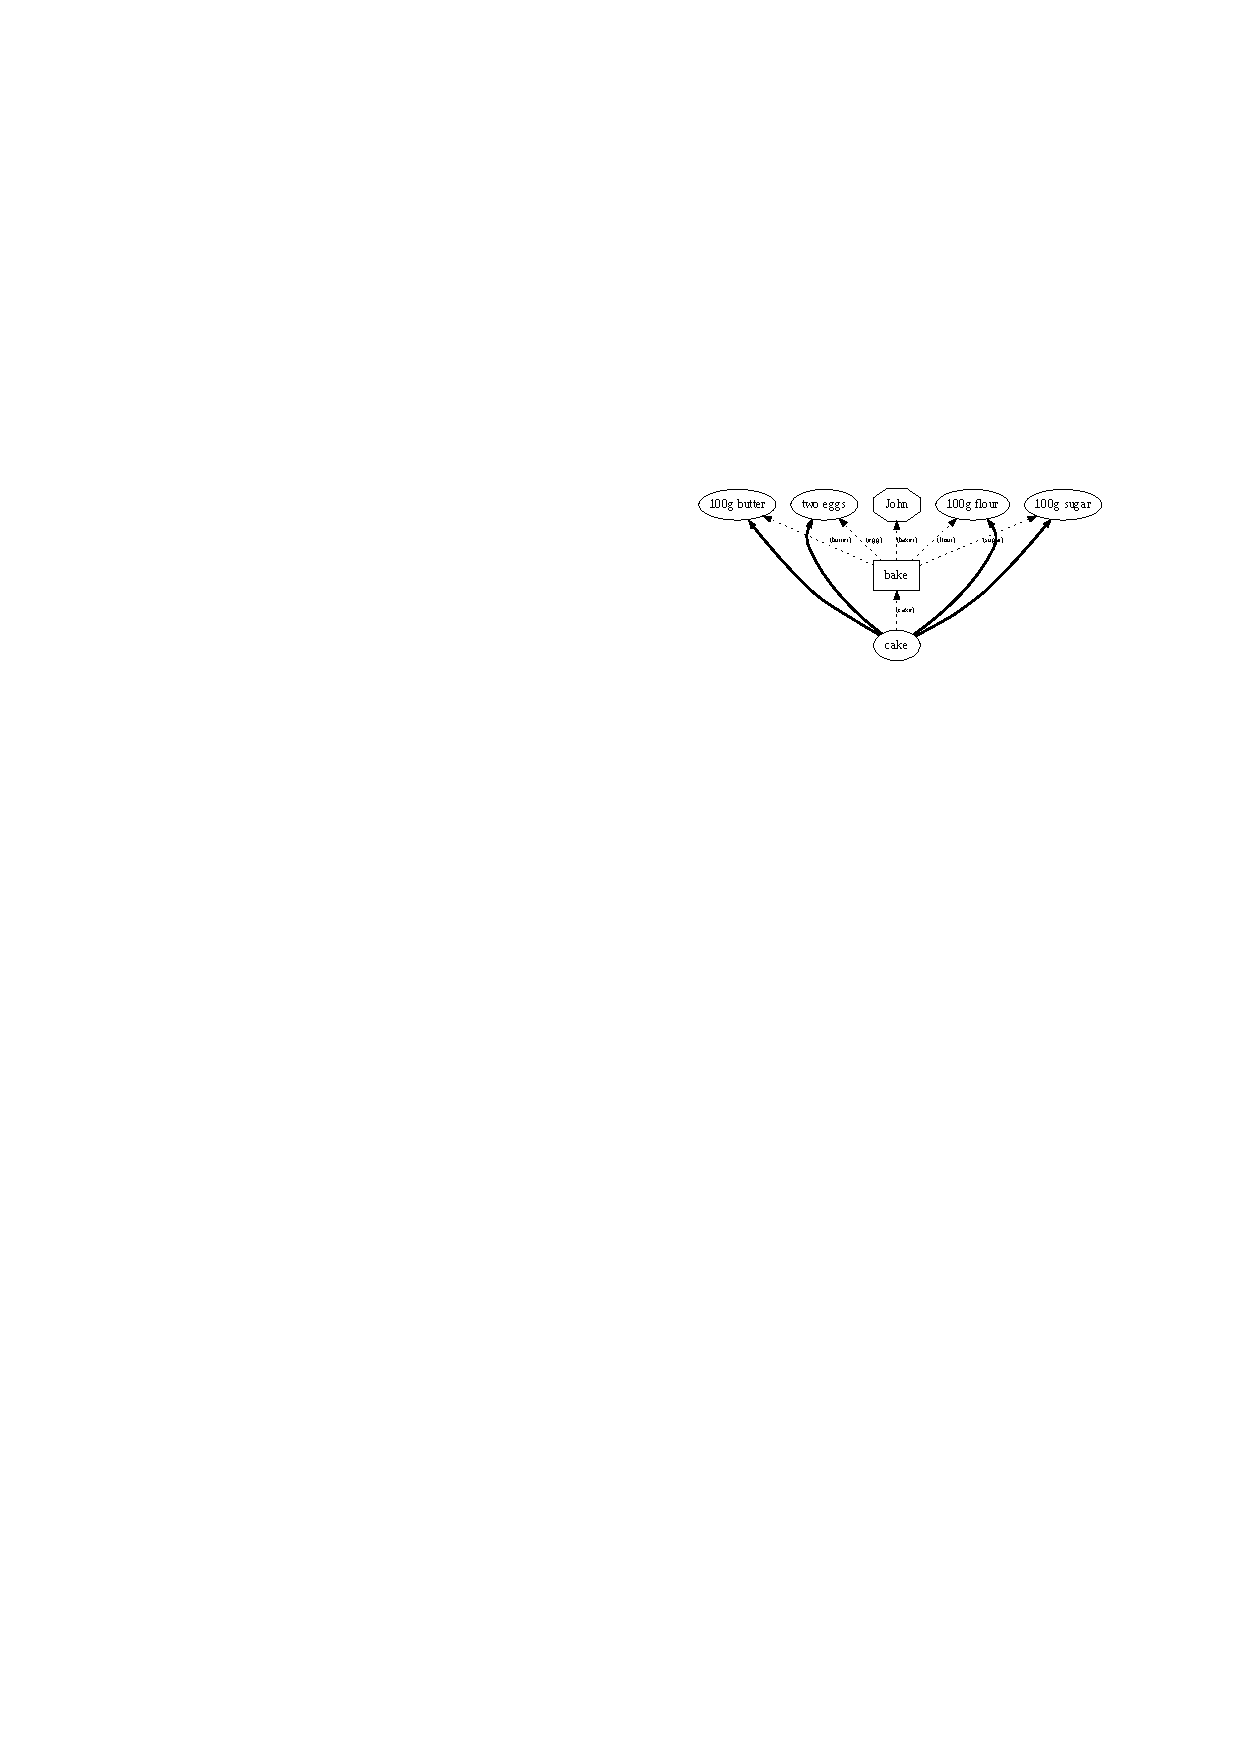
\includegraphics[width=\linewidth]{provenance-graph}
	\caption{A provenance graph for ``cake baking'' using the Open Provenance Model. The cake (artifact) was baked (the process) by John (the agent) using ingredients including butter, eggs, flour and sugar (artifacts). \is{Moreau2011}}
	\label{fig:lr-provenance-graph}
\end{figure}

The Open Provenance Model is general and can be extended in both the structure and vocabulary to represent domain-specific problems. ProveML~\cite{Walker2013} is an extension of this model for recording the provenance of data, analytical process and interpretations in human terrain visual analytics.

\subsection{Analytic Provenance}
Definition from ~\cite{North2011}, our agenda~\cite{Xu2015}

\subsubsection{Model}
Modeling of analytic provenance: 4-level model by Gotz and Zhou and other vis task/action taxonomies such as classic Shneiderman's task by data type~\cite{Shneiderman1996}, Amar's low-level~\cite{Amar2005}, Amar's high-level~\cite{Amar2004}, more recent Bhemer's typology what-why-how~\cite{Brehmer2013}.

\subsubsection{Capture}
combine previous reviews from the draft survey of analytic provenance, research agenda, and capture in the context of online sensenmaking the last paper